\chapter[Modeling the spatial density of vents in volcano clusters on Earth, Mars, and Venus]{Modeling the spatial density of vents in volcano clusters on Earth, Mars, and Venus}\label{ch_kde}

\renewcommand*{\FigPath}{figures/chapter-spatial_density}

\section{Abstract}
The spatial density of volcanic vents in 20 distributed volcano clusters on three different planets has been modeled, including 10 volcanic fields on Earth, 3 fields on Mars, and 4 shield fields and 3 shield plains on Venus. Vent density for clusters is characteristic on a planetary scale, with vent density being highest at Earth clusters (0.1 vents~km$^{-2}$), lowest at Mars clusters (0.001 vents~km$^{-2}$), and intermediate in Venus clusters (0.01 vents~km$^{-2}$). The widths of the probability density functions used to model vent density are known as the Kernel Bandwidth, and are modeled independently for each volcano cluster. Bandwidth orientation and elongation is used as a proxy of cluster orientation and elongation, and might be influenced by underlying characteristics of the lithosphere or the magma source region. Bandwidth characteristics are compared in regions where elongated source regions are expected, where the source region might have migrated over time, and where lithospheric features might enable or inhibit magma focusing in different directions.

\section{Introduction}

Physical processes in nature often create a partially random set of point features, such as sinkholes, volcanoes, or kettle lakes. The spatial distribution of these features is governed by one or more physical processes, which may be modeled to create a statistical description of where points are more likely to occur. For instance, sinkholes are more likely to occur in locations where soluble carbonate rock is at or near the water table, so a map showing the probability of sinkhole development might reflect the distribution of shallow carbonate rocks. In volcanically active regions, volcanoes are formed from a magma source. If the location, depth, and productivity of the magma source is well known, models can be made to map the potential locations of volcanism on the surface, where a higher likelihood of eruption would be over the most productive locations of the magma source. 

The distribution and characteristics of magma sources in the ground, however, are far less constrained than the distribution of volcanoes on the Earth's surface. Instead of creating a probabilistic spatial model of volcanic events using knowledge of the magma source, the existing distribution of volcanoes is used \citep{connor2015probabilistic,germa2013tectonic}. Using only the point locations of volcanoes, one might conclude that new volcanoes are likely to form in areas where volcanoes already exist, or where the number of volcanoes per unit area is higher. Using point locations to create a statistical model of volcano production is an attempt to model one aspect of a magma generation and ascent, when knowledge of the physical processes may be limited.

In this Chapter, vent density is modeled as a 2D probability density function (PDF) that integrates to $\lesssim$1 over the volcanic field. This means that, for active volcano clusters, any new vent has a $\sim$100\% chance of being created in the same general area as the current field. The ``vent intensity function'' is defined as the probability density function of a volcano cluster multiplied by the number of vents cataloged in the cluster. This intensity function integrates to the number of cataloged vents, so the ``vent intensity'' of an area has the units of vents/km$^2$.

Vent density has been modeled for 20 volcano clusters on the Earth, Mars, and Venus. The clusters of each planet are compared based on number of vents, areal footprint, and average vent intensity, in order to identify the variation of distributed volcanism on each planet and discern any clear differences between clusters on each planet. Patterns in the vent density function of selected clusters are also examined. Elongation of volcano clusters can be attributed to the orientation of fractures in the elastic layer of the lithosphere \citep{delaney1986field}, geodynamic stress \citep{germa2013tectonic}, migration of a magma source \citep{richardson2013volcanic, tanaka1986migration} or elongation of the magma source \citep{tamura2002hot}. One aspect of the vent density function, the kernel bandwidth (defined in Section \ref{sec_kde}) will be used as a proxy for vent field orientation and elongation. Kernel bandwidths for different clusters will be compared to geologic features that are known or are hypothesized to focus magma under their corresponding volcano cluster.

\subsection{Estimating vent intensity} 
A simple estimate of vent intensity can be carried out by counting the number of volcanoes in each 1~km by 1~km cell of a rectangular grid laid over all the vents in a volcano cluster \citep{lutz1995improved} (or a grid of any tesselating shape \citep{glaze2005statistical}). Because vents in most clusters are spaced multiple km from each other, however, this would result in a grid of mostly 0 or 1 vents/km$^2$, which would appear similar to a map of vent locations drawn as points. Another disadvantage to this approach is that sharp lines delineate the change in vent density. On one side of a grid cell boundary, the vent density might be 1 vent/km$^2$, while one meter away density might rapidly decrease 100\% to 2 vents/km$2$. In nature, however, it is unlikely that a volcano is twice as likely to erupt in one square meter compared to its adjacent square meter.

An alternative method to measure spatial vent density would be to assign a search radius to each point location on a map. Here the spatial vent density is the number of vents within the radius divided by the area of the circle defined by the search radius \citep{connor1987structure,connor1990cinder}. This effectively smooths vent density if the search radius is increased to several km since the range to which each vent influences the density model increases. While this model might be an improvement over the grid method above, it still has the same problem of sharp changes in vent density at locations within one search radius's distance from a vent. 

Because the goal of modeling vent density is to identify an underlying probabilistic model of vent creation, it is important to select a method that avoids these artificially sharp density changes \citep{connor1995three}. The method used should also be able to be validated using known distributions and point samples from these distributions. A third method of estimating spatial density avoids sharp density changes by substituting the search radius with a probability density function, centered on each vent location.

\subsection{Kernel density estimation}\label{sec_kde}
The process of estimating the ``true'' point density distribution by assigning probability density functions (PDFs) to a population of randomly sampled points from this distribution is called Kernel Density Estimation (KDE) \citep{silverman1986density}. A kernel is an identical PDF assigned to points to describe their influence on the surrounding region. Essentially, if the kernel is the normal distribution centered on a point, the point has more influence at the point's location (at the maximum value of the normal distribution). Influence decreases away from the point following the value of the normal distribution \citep{lutz1995improved}. In KDE, density is modeled as influence, so that point density is highest at a point location and decreases away from the point, in effect smoothing the point.

Given a map catalog of volcanoes, a density value, $\lambda$, for each volcano can be calculated for any location on the map using the associated kernel PDF. If the kernel is normally distributed \citep{conway1998recurrence}, the kernel density of a volcano for location with Cartesian coordinates ($x$,$y$) is calculated as
\begin{equation}
\lambda(x,y) = \frac{1}{\sigma\sqrt{2\pi}}\exp\left[\frac{-(x-x_v)^2-(y-y_v)^2}{2\sigma^2}\right]
\end{equation}
where ($x_v$,$y_v$) is the coordinate pair of the volcano and $\sigma$ is the PDF standard deviation, or kernel bandwidth. The larger the kernel bandwidth, the further the density of the point is spread across the map \citep{lutz1995improved}. The total volcano point density at this location can be found by summing the point densities of all volcanoes, $i$, in the catalog of $N$ volcanoes:
\begin{equation}
\lambda(x,y) = \frac{1}{N\sigma\sqrt{2\pi}}\sum\limits_{i=1}^{N}\exp\left[\frac{-(x-x_i)^2-(y-y_i)^2}{2\sigma^2}\right].
\label{eq_simpleKDE}
\end{equation}

By calculating vent density for all locations in an area, a continuous, differentiable surface is produced, which is the modeled density function for the cluster. Note that in Equation \ref{eq_simpleKDE} the entire formula is divided by the number of vents, $N$. Integrating $\lambda$ over the x and y domains in Equation \ref{eq_simpleKDE} then results in unity \citep{connor2015probabilistic}; given an eruption, there is a probability of 1 that the eruption will take place somewhere on the surface of the planet. This means that $\lambda$ is treated as a 2D probability density function with units of m$^{-2}$. Vent intensity with units of vents~m$^{-2}$ can be found by multiplying the $\lamba$ density curve by $N$.

Kernel PDFs do not have to be axi-symmetric normal distributions. In this paper, a bivariate normal distribution will be used to model density, so kernels will be Gaussian ellipses instead of circles (circular distributions can be considered univariate as they are defined by one standard deviation or bandwidth). These ellipses will also be unconstrained in direction, so their major axes do not have to be aligned in a cardinal direction \citep{wand1993comparison}. This is done by multiplying the distance between locations and volcanoes, treated here a 1x2 distance matrix, by a covariance matrix that defines the standard deviation in the x and y directions and the covariance between these dimensions. The covariance matrix is given as
\begin{equation}\begin{bmatrix}
\sigma_x^2 & \sigma_x\sigma_y\rho\\
\sigma_x\sigma_y\rho & \sigma_y^2
\label{eq_covariance}
\end{bmatrix}\end{equation}
where $\sigma_x$ is the x-direction standard deviation, $\sigma_y$ is the y-direction standard deviation, and $\rho$ is the correlation of these two. A correlation of 0 results in a kernel ellipse with axes aligned with the cardinal directions, while higher correlation skews or rotates the ellipse away from the cardinal directions \citep{wand1993comparison}.

Kernel bandwidth, the amount that the kernel ellipse is smoothed in any given direction, is an important parameter in estimating the unknown density of point features \citep{lutz1995improved,connor2015probabilistic}. Again, the point of KDE is to estimate the underlying spatial probability of a point feature (e.g. a volcano) being created, using only the points that can already be observed \citep{connor2000geologic}. Selecting a bandwidth that is too small will overly concentrate volcano density around each existing volcanoes, underestimating the likelihood of a new volcano in between existing edifices. A bandwidth that is too large will overly smooth volcano density, overestimating the likelihood of new volcanic events far from the existing volcano population.

Several bandwidth selectors have been created for KDE. In this project the Summed Asymptotic Means Square Error (SAMSE) selector will be used \citep{duong2007}. This selector is chosen because it has been validated using point populations of known distributions and it has been shown to be more stable than similar selectors \citep{duong2003}. The SAMSE bandwidth selector also is preferred because it provides an unconstrained bandwidth model using the covariance matrix formula in Equation \ref{eq_covariance}.

Calculating the estimated spatial density, $\hat{\lambda}$, of point features in a location, $s$, using the unconstrained, bivariate bandwidth is done by modifying Equation \ref{eq_simpleKDE}, so that
\begin{equation}
\hat{\lambda}(\mathbf{s})=\frac{1}{2N\pi\sqrt{|\mathbf{H}|}}\sum\limits_{i=1}^{N}\exp\left[-\frac{1}{2}\mathbf{b^Tb}\right]
\label{eq_kde}
\end{equation}
where $\mathbf{H}$ is the 2x2 covariance matrix and $|\mathbf{H}|$ is its determinant, $\mathbf{b}=\mathbf{H}^{-0.5}\mathbf{d}$ and $\mathbf{b^T}$ is its transpose. $\mathbf{d}$ is the 1x2 distance matrix, with the form
\begin{equation}\begin{bmatrix}
x_s-x_i\\
y_s-y_i
\label{eq_distancematrix}
\end{bmatrix}\end{equation}
where ($x_s$,$y_s$) are the Cartesian coordinates of the location of interest and ($x_i$,$y_i$) are the coordinates of the $i^{\text{th}}$ volcano \citep{connor2015probabilistic}.

Here, volume density is also modeled by including a list of weights for each volcanic vent, where weights are eruption volumes of the volcanoes. Weighting the density functions corresponding to each volcanic vent requires expanding Equation \ref{eq_kde} to include weights, $\omega$, as follows.
\begin{equation}
\hat{\lambda}_{vol}(\mathbf{x,y})=\frac{1}{2\pi\sqrt{|\mathbf{H}|}\sum{\omega}}\sum\limits_{i=1}^{N}\left(\exp\left[-\frac{1}{2}\mathbf{b^Tb}\right]\omega_i\right)
\label{eq_weigthedkde}
\end{equation}
This function is normalized to unity by including the sum of all weights in the denominator instead of the number of point locations. In Equation \ref{eq_kde}, the number of locations is used, as all points are weighted equally (i.e. their weights are each equal to 1). Volume intensity, with units km$^3$~km${-2}$, is the product of the volume density function and the total volume of volcanoes in the catalog.

%bu zhi da
\section{Methods}

\subsection{Data collection}
Catalogs of 20 volcano clusters have been collected for this study, including 10 volcanic fields on Earth, 3 on Mars, and 7 on Venus. The clusters are each distributed volcanic fields and volcanoes in them are likely monogenetic. Some clusters are formed nearby or on top of central-vent volcanoes (e.g. Mount Adams, WA and Arsia Mons, Mars), though most are not associated with large volcanoes and can be described as ``plains-style'' \citep{greeley1977basaltic} or ``planform'' \citep{settle1979structure} fields. 

Each cluster catalog includes the locations of volcanic vents that are presently observable in the area. Volcanic vents are generally located at the center of scoria cones, low shields, or tuff rings and are often depressions in the center of topographic rises. Scoria cones, low shields, and tuff rings in these fields are $<1$ to a few km in diameter and are interpreted to be the products of monogenetic volcanic eruptions. One cluster, the San Rafael volcanic field, is heavily eroded to a depth of $\sim$1~km so no edifices remain. In this cluster, diabasic conduit diatremes are mapped and interpreted to be vent locations.

The locations of each volcanic vent are defined as 2D points on their planet's surface, even though volcanic vents are not precisely point features. A vent location point generally describes the center location of the vent. Points are not defined by the center of the volcano edifice, because they are used to identify the location where magma intersected and erupted onto the planet's surface, often as a dike. This point feature can then be used in the KDE method to model volcanic vent density.

\begin{figure}
\centering
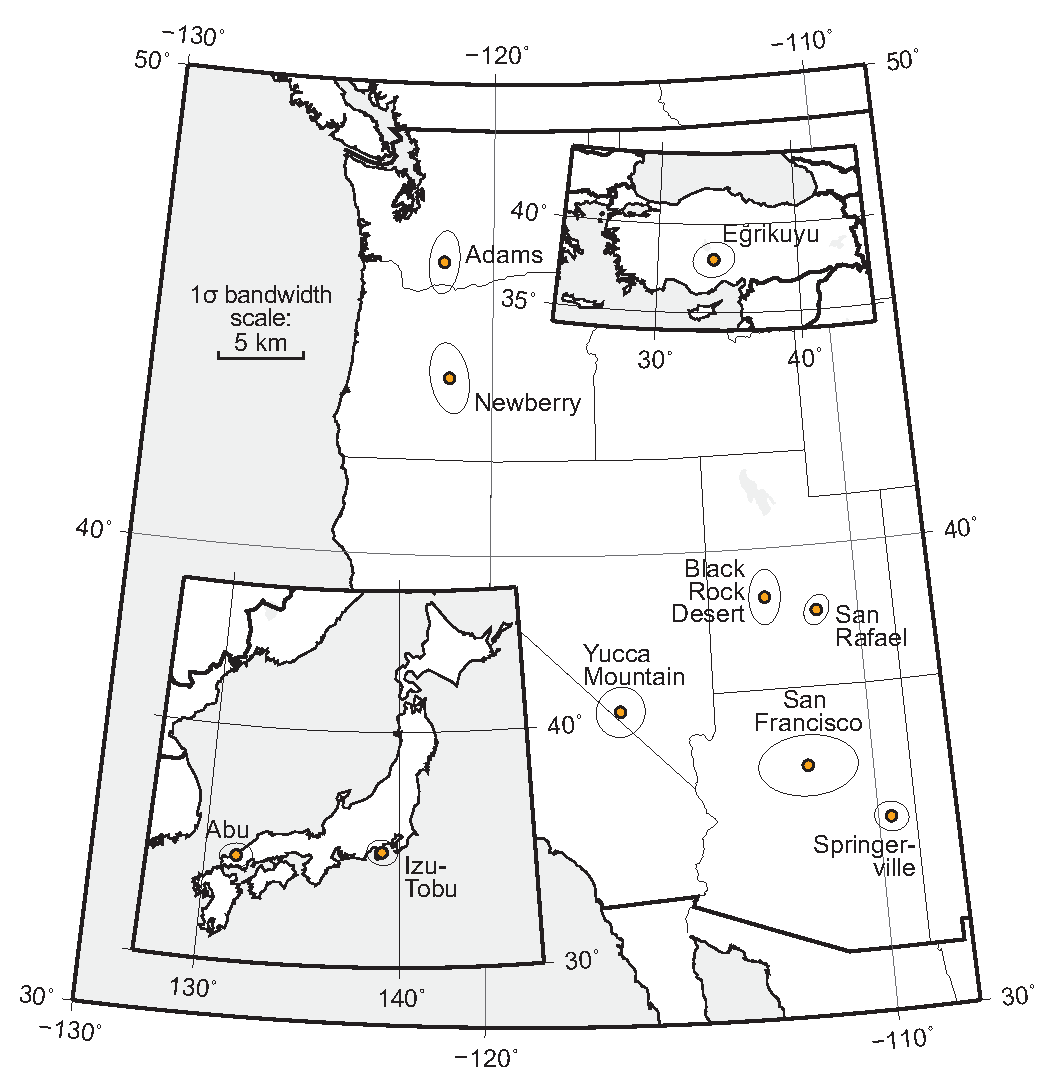
\includegraphics[width=0.5\linewidth]{\FigPath/locators/earth_locator.eps}
\caption[Locations of selected volcano clusters on Earth]{Locations of selected volcano clusters on Earth. Kernel bandwidth ellipses are drawn over each location. Ellipses are enlarged to show regional variation.}
\label{fig_earthlocator}
\end{figure}

\subsubsection{Earth clusters}
Ten distributed-style volcanic fields on Earth have been mapped, producing vent catalogs that can be used to model vent density in the region. These clusters are located in distinct tectonic settings: over subduction zones, on the Colorado Plateau, in the extensional Basin and Range region, and in the Anatolian Peninsula (Figure \ref{fig_earthlocator}).

\paragraph{Subduction-related clusters} 
Distributed volcanic fields in the Cascades Arc have formed in association with the large central volcanoes, including Mount Adams \citep{barron2014database} and Newberry Volcano \citep{bard2013database}. This arc is the product of the subducting Juan de Fuca plate. In southern Japan, monogenetic volcano groups have also formed, due to subduction of the Phillipines and Pacific plates. Two of these volcano groups, the Abu Monogenetic Volcano Group and the Izu-Tobu Volcano Group have been mapped in this region \citep{kiyosugi2010relationships} and vent density has been modeled by \citet{kiyosugi2012relationship} Edifices in these catalogs are scoria cones, low shield volcanoes, and lava domes.

\paragraph{Colorado Plateau} Basaltic volcanism has occurred as an annulus around the Colorado Plateau during the Cenozoic \citep{tanaka1986migration}. Most of this volcanism is distributed in style, forming isolated volcano clusters. Three of these clusters, the San Francisco Volcanic Field (SFVF), Black Rock Desert, and the San Rafael Volcanic Field, are included in this study. 

Volcanic vents in the SFVF, located in and around Flagstaff, AZ, have been cataloged by \citet{harburger2014probabilistic}, including 583 vents identified as monogenetic. This field has been active for three magnetic epochs, enabling separation into three sub-fields which can be independently analyzed \citep{tanaka1986migration}. Black Rock Desert volcanoes in Utah were cataloged by \citet{hintz2008physical} and vent density has been modeled by \citet{kiyosugi2012relationship}. \citet{kiyosugi2012relationship} also mapped 126 conduits diatremes in the heavily eroded San Rafael Volcanic Field in central Utah and interpreted these to be previous vent locations when the field was active in the Pliocene.

\paragraph{Other tectonic settings} Two other vent databases have been created for clusters in the Basin and Range, Nevada, and in Central Anatolia, Turkey. In the Basin and Range, \citet{connor1995three} cataloged 39 scoria cones located in a cluster around Yucca Mountain. In Central Anatolia, \citet{uslular2015size} mapped 77 scoria cones, which form the E\u{g}rikuyu volcano cluster. The volume of each scoria cone is also reported by \citet{uslular2015size}.

\begin{figure}
\centering
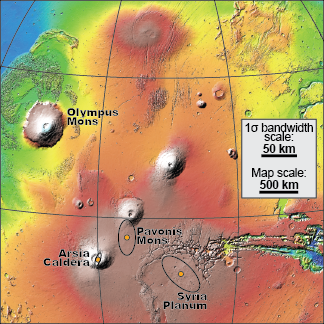
\includegraphics[width=0.5\linewidth]{\FigPath/locators/mars_locator_72dpi.png}
\caption[Locations of selected Martian volcano clusters in the Tharsis Volcanic Province]{Locations of selected Martian volcano clusters in the Tharsis Volcanic Province. Kernel bandwidth ellipses are drawn at the 1$\sigma$ contour over them. Ellipses are enlarged.}
\label{fig_marslocator}
\end{figure}

\subsubsection{Mars clusters}
Three distributed-style volcanic fields within the larger Tharsis Province are included in this study: Syria Planum, Southern Pavonis Mons, and Arsia Mons Caldera. The Tharsis Volcanic Province has  been identified as a long lived center for volcanism since early space missions to Mars \citep{carr1977some} and makes up about one-quarter of the total global surface. Tharsis is home to many of the largest central-vent style volcanoes in the Solar System, but also has over 1,000 small volcanic vents that are distributed in clusters around Tharsis.

Three clusters of vents have been identified in the southern Tharsis region that are separated from other vents in the database and are treated as isolated populations because of this (Figure \ref{fig_marslocator}). Each field, Syria, Pavonis, and Arsia, were potentially formed from one magma generation event, though they might have also been formed from multiple events that created overlapping volcano clusters.

\paragraph{Southern Pavonis Mons}
Pavonis Mons is a large shield volcano in the Tharsis Montes, a linear chain of three shield volcanoes within the Tharsis Province. To the north and south of each of these volcanoes, lavas have been emplaced on the shield flank, apparently after the main construction phases of each shield \citep{bleacher2007tharsis}. These lavas are known as flank aprons \citep{bleacher2007tharsis}. At Pavonis, a volcano cluster of 88 shield volcanoes (one to tens km in diameter) is present on top of the southern flank apron \citep{bleacher2009spatial}. This cluster is aligned roughly N-S along the axis of the apron \citep{bleacher2009spatial}.


\paragraph{Arsia Mons Caldera}
Arsia Mons is the southernmost large shield volcano of the Tharsis Montes and has a 110~km diameter caldera at its summit. Within this caldera, 29 low shield volcanoes have been mapped [Chapter 4, this dissertation]. The caldera and shields within it are thought to be very young due to the absence of any impact craters larger than 1~km in the entire caldera \citep{crumpler1996calderas}. In addition to the 29 vent locations, volumes have been modeled for the lavas effused from each vent using an interpolated subsurface model for each lava flow [Chapter 4, this dissertation]. These volume estimates will be used to compare the spatial vent density of the field to a volume-weighted spatial density model.

\paragraph{Syria Planum}
The Syria Planum region is a broad plateau with 263 low shield volcanoes \citep{richardson2013volcanic}. One volcano, Syria Mons, has lava flows that travel up to 1,000~km from its vent \citep{baptista2008swarm}. The other low shields have been mapped by \citet{richardson2013volcanic} and are one to tens of km in diameter with slopes of $<6^{\circ}$. This volcano cluster has been dated using crater retention rate models to have formed between 3.6-2.9~Ga spanning the Hesperian geologic period on Mars.

\begin{figure}
\centering
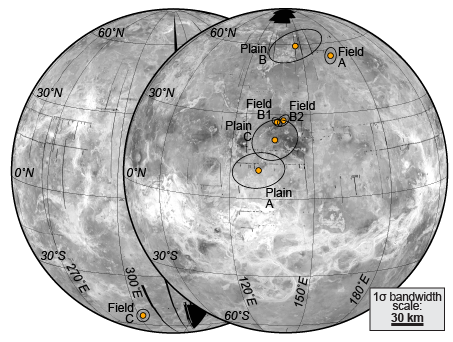
\includegraphics[width=0.6\linewidth]{\FigPath/locators/venus_globe_72dpi.png}
\caption[Locations of seven volcano clusters on Venus]{Locations of seven volcano clusters on Venus. Kernel bandwidth ellipses are drawn at the 1$\sigma$ contour over each cluster and are enlarged.}
\label{fig_venuslocator}
\end{figure}

\subsubsection{Venus clusters}
Seven Venus clusters have been cataloged by \citet{miller2012shield}, which fall into two distinct classes: four are ``shield fields'' which are composed of $10^3$-$10^4$ volcanic vents and three are ``shield plains'' which host $10^4$-$10^5$ volcanic vents (Figure \ref{fig_venuslocator}). Both types of cluster are formed by low sloped (less than one to a few degrees) shields $<$10~km in diameter \citep{richardson2012comparison}. These shields are radar bright or dark, enabling their mapping with left-look Magellan radar images, though their vents are often not visible, so vents are mapped as the centroid of the edifice \citep{miller2012shield}. Of the seven clusters cataloged, three are shield plains and four are shield fields \citep{miller2012shield}.

The large size difference between shield fields and shield plains has been observed since the return of Magellan radar images \citep{head1992venus}. Venusian shield fields are similar in size to the shield fields on Mars and have a similar number of vents (several hundreds) to fields on Mars and Earth. Venusian plains, however, are regional in scale and include several thousand vents. The Venusian surface has very few impact craters, indicating that it has recently been resurfaced. The regional volcanic plains would have played an important role in this resurfacing, due to their large footprints \citep{guest1992small}.

\begin{table}[t!]
\centering
\caption{Distributed-style Volcano Clusters on Earth}
\begin{tabular}{p{2cm} p{2.5cm} p{2cm} c c p{4cm}}
\toprule
Cluster	&	Region, &	Location	&	Vent &	Bandwidth	&	Data\\
Name		& Country	&	Lat, Long	&	Count	&	Matrix (km$^2$)	&Source\\
\midrule
Abu$^*$		&	Ch\={u}goku, Japan	&	34$^{\circ}$30'N, 131$^{\circ}$35'E	&	56	&	$\bigl[\begin{smallmatrix} 3.81&0.230\\0.230&2.05 \end{smallmatrix}\bigr]$	&	\citet{kiyosugi2012relationship,kiyosugi2010relationships}\\
Adams		&	Washington, USA	&	46$^{\circ}$10'N, 121$^{\circ}$30'W	&	89	&	$\bigl[\begin{smallmatrix} 3.25&0.989\\0.989&13.9 \end{smallmatrix}\bigr]$	&	\citet{barron2014database}\\
Blk. Rock Desert$^*$ &	Utah, USA		&	39$^{\circ}$N, 112$^{\circ}$30'W&	39	&	$\bigl[\begin{smallmatrix} 3.51&0.500\\0.500&10.6 \end{smallmatrix}\bigr]$	&	\citet{kiyosugi2012relationship,hintz2008physical}\\
E\u{g}rikuyu	&	Central Turkey	&	34$^{\circ}$N, 38$^{\circ}$E	&	77	&	$\bigl[\begin{smallmatrix} 10.8&1.00\\1.00&7.57 \end{smallmatrix}\bigr]$	&	\citet{uslular2015size}\\
Izu-Tobu$^*$	&	Ch\={u}bu, Japan	&	35$^{\circ}$N, 139$^{\circ}$20'E	&	126	&	$\bigl[\begin{smallmatrix} 3.29&-0.200\\-0.200&2.27 \end{smallmatrix}\bigr]$	&	\citet{kiyosugi2012relationship}\\
Newberry	&	Oregon, USA	&	43$^{\circ}$45'N, 121$^{\circ}$15'W	&	327	&	$\bigl[\begin{smallmatrix} 5.57&-2.43\\-2.43&17.3 \end{smallmatrix}\bigr]$	&	\citet{bard2013database}\\
San \mbox{Francisco}	&	Arizona, USA	&	35$^{\circ}$20'N, 111$^{\circ}$50'W	&	583	&	$\bigl[\begin{smallmatrix} 34.4&-0.0396\\-0.0396&13.0 \end{smallmatrix}\bigr]$	&	\citet{harburger2014probabilistic}\\
San Rafael	&	Utah, USA	&	38$^{\circ}$35'N, 111$^{\circ}$15'W	&	63	&	$\bigl[\begin{smallmatrix} 2.31&0.720\\0.720&3.12 \end{smallmatrix}\bigr]$	&	\citet{kiyosugi2012relationship}\\
Springerville &	Arizona, USA	&	34$^{\circ}$15'N, 109$^{\circ}$45'W	&	400	&	$\bigl[\begin{smallmatrix} 4.07&-0.300\\-0.300&3.14 \end{smallmatrix}\bigr]$	&	\citet{kiyosugi2012relationship,condit2010dynamic}\\
Yucca Mountain$^*$ &	Nevada, USA	&	36$^{\circ}$40'N, 116$^{\circ}$30'W	&	39	&	$\bigl[\begin{smallmatrix} 8.35&0.42\\0.42&8.75 \end{smallmatrix}\bigr]$	&	\citet{kiyosugi2012relationship,connor1995three}\\
\bottomrule
\multicolumn{6}{p{0.95\linewidth}}{$^*$ Cluster data (including bandwidth matrix) are reported in \citet{kiyosugi2012relationship}, but vent locations are not included in this report.}\\
\label{tab_clusterdataE}
\end{tabular}
\end{table}

\subsection{Estimating vent density with the KDtools Python Library}

A Python library has been created to map the spatial density of geographic points, with specific functions to deal with geographic projections on Earth, Mars, and Venus. This library, called KDtools (Kernel Density Tools), contains seven functions which can be used to pre-process data, identify an optimal kernel bandwidth of the data, evaluate the local point density for locations on a map, and export these results to a raster file. Each function code is given in Appendix \ref{apdx_kdtoolsmaps}. Two functions, explained below, are used to first identify an optimal kernel bandwidth, and second to evaluate the spatial density of points across a map grid.

\begin{table}[t!]
\centering
\caption{Distributed-style Volcano Clusters on Venus and Mars}
\begin{tabular}{p{2cm} p{2.5cm} p{2cm} c c p{4cm}}
\toprule
Cluster	&	Region, &	Location	&	Vent &	Bandwidth	&	Data\\
Name		& Country	&	Lat, Long	&	Count	&	Matrix (km$^2$)	&Source\\
\midrule
Field-A	&	Atalanta, Venus	&	54$^{\circ}$N, 168$^{\circ}$E	&	344	&	$\bigl[\begin{smallmatrix} 115&7.74\\7.74&238 \end{smallmatrix}\bigr]$	&	\citet{miller2012shield}\\
Field-B1	&	Vellamo, Venus	&	27$^{\circ}$N, 137$^{\circ}$E	&	135	&	$\bigl[\begin{smallmatrix} 88.7&-35.4\\-35.4&71.4 \end{smallmatrix}\bigr]$	&	\citet{miller2012shield}\\
Field-B2	&	Vellamo, Venus	&	328$^{\circ}$N, 139$^{\circ}$E	&	169	&	$\bigl[\begin{smallmatrix} 125&51.7\\51.7&116 \end{smallmatrix}\bigr]$	&	\citet{miller2012shield}\\
Field-C	&	Mylitta, Venus	&	52$^{\circ}$S, 58$^{\circ}$W	&	290	&	$\bigl[\begin{smallmatrix} 140&2.93\\2.93&138 \end{smallmatrix}\bigr]$	&	\citet{miller2012shield}\\
Plain-A	&	Greenaway, Venus	&	11$^{\circ}$N, 130$^{\circ}$E	&	2919	&	$\bigl[\begin{smallmatrix} 2440&164\\164&1120 \end{smallmatrix}\bigr]$	&	\citet{miller2012shield}\\
Plain-B	&	Atalanta, Venus	&	60$^{\circ}$N, 150$^{\circ}$E	&	10225	&	$\bigl[\begin{smallmatrix} 2470&709\\709&1000 \end{smallmatrix}\bigr]$	&	\citet{miller2012shield}\\
Plain-C	&	Greenaway, Venus	&	20$^{\circ}$N, 135$^{\circ}$E	&	3460	&	$\bigl[\begin{smallmatrix} 1860&232\\232&1460 \end{smallmatrix}\bigr]$	&	\citet{miller2012shield}\\
Arsia		&	Tharsis, Mars	&	9$^{\circ}$S, 120$^{\circ}$W	&	29	&	$\bigl[\begin{smallmatrix} 81.4&105\\105&347 \end{smallmatrix}\bigr]$	&	Chapter \ref{ch_arsia}\\
Pavonis	&	Tharsis, Mars	&	4$^{\circ}$S, 114$^{\circ}$W	&	89	&	$\bigl[\begin{smallmatrix} 579&-0.616\\-0.616&2520 \end{smallmatrix}\bigr]$	&	\citet{bleacher2009spatial}\\
Syria		&	Tharsis, Mars	&	14$^{\circ}$S, 100$^{\circ}$W	&	263	&	$\bigl[\begin{smallmatrix} 2810&-1720\\-1720&2620 \end{smallmatrix}\bigr]$	&	\citet{richardson2013volcanic}\\
\bottomrule
\multicolumn{6}{p{0.95\linewidth}}{$^*$ Cluster data (including bandwidth matrix) are reported in \citet{kiyosugi2012relationship}, but vent locations are not included in this report.}\\
\label{tab_clusterdataVM}
\end{tabular}
\end{table}

\begin{table}
\centering
\caption[Sub-populations of the San Francisco Volcanic Field]{Sub-populations of the San Francisco Volcanic Field$^*$}
\begin{tabular}{l c p{2cm} c c}
\toprule
Magnetic	&	Time Span	& Centroid	&	Vent &	Bandwidth\\
chronozone		&	Ma	& Lat, Long	&	Count	&	Matrix (km$^2$)\\
\midrule
Brunhes	&	0.73 - Present	&	35$^{\circ}$20'N, 111$^{\circ}$30'W	&	239	&	$\bigl[\begin{smallmatrix} 21.6&-5.66\\-5.66&11.7 \end{smallmatrix}\bigr]$\\
Matuyama	&	2.48 - 0.73	&	36$^{\circ}$20'N, 112$^{\circ}$W	&	209	&	$\bigl[\begin{smallmatrix} 15.0&1.38\\1.38&25.4 \end{smallmatrix}\bigr]$\\
Pre-Matuyama	&	5-2.48	&	36$^{\circ}$20'N, 112$^{\circ}$15'W	&	135	&	$\bigl[\begin{smallmatrix} 13.3&-3.10\\-3.10&12.5 \end{smallmatrix}\bigr]$\\
\midrule
Entire Field	&	5 - Present	&	35$^{\circ}$20'N, 111$^{\circ}$50'W	&	583	&	$\bigl[\begin{smallmatrix} 34.4&-0.0396\\-0.0396&13.0 \end{smallmatrix}\bigr]$\\
\bottomrule
\multicolumn{5}{p{0.95\linewidth}}{$^*$Vent locations reported in \citet{harburger2014probabilistic}.}\\
\label{tab_sfvfdata}
\end{tabular}
\end{table}

The kernel bandwidth is determined with the SAMSE method in the \textbf{samse\_bandwidth} function, by calling the R statistical language in which the SAMSE bandwidth selector has been programmed. The single input of this function is the list of locations of each volcanic vents projected in meter units. A $2\times 2$, unconstrained covariance matrix is returned from this function.

Local vent density is calculated along a grid in the function \textbf{KD} with the covariance matrix defining the Gaussian kernel ellipse. The smoothed density of each vent is calculated over the grid locations given their distance from the vent. This density is then added to the total density at each location in order to form the summation shown in Equation \ref{eq_kde}. After the density functions attributed to all vents have been calculated over the grid, all density values are normalized with the left half of Equation \ref{eq_kde}. The output of this function is a 2-dimensional array of density values corresponding to the grid surrounding vent locations. The sum of these density values approaches 1.0 as the grid size is increased around the volcano cluster. Volume density can also be modeled with function \textbf{KD} by providing weights to the function, following Equation \ref{eq_weigthedkde}.

\section{Results}
The locations, vent counts, and kernel bandwidth matrices for each volcano cluster are reported in Tables \ref{tab_clusterdataE} and \ref{tab_clusterdataVM}. Data and results for four clusters, Abu Monogenetic Volcano Group, Izu-Tobu Monogenetic Volcano Group, Black Rock Desert, and the Yucca Mountain Volcano Group are duplicated in Table \ref{tab_clusterdataE} from \citet{kiyosugi2012relationship}. In addition to modeling vent density for the entire field, vent density is modeled for each paleomagnetic sub-group in the San Francisco Volcanic Field. Vent count and bandwidth matrices are listed separately in Table \ref{tab_sfvfdata}. Maps of vent density for volcano clusters on Earth, Mars, and Venus are shown in several figures below as well as Appendix \ref{apdx_kdtoolsmaps}.

\begin{figure}
\centering
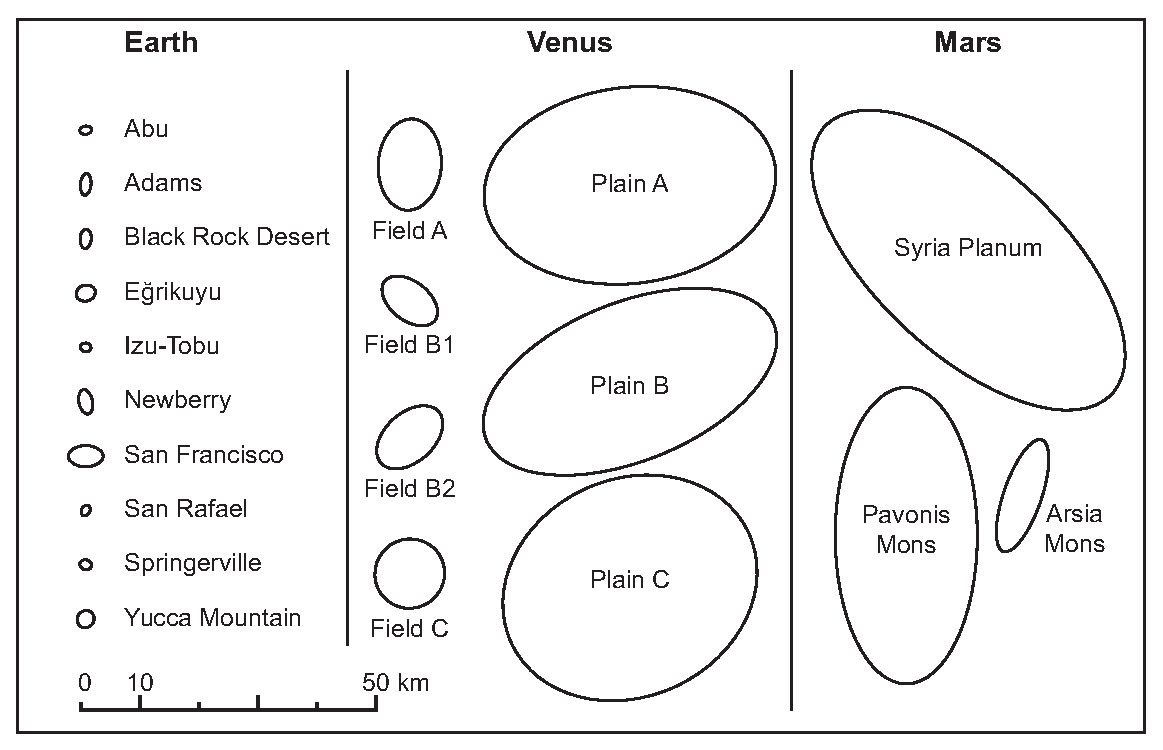
\includegraphics[width=0.7\linewidth]{\FigPath/Kernel-Ellipses.eps}
\caption[Kernel bandwidth ellipses for different clusters on Earth, Venus, and Mars]{Kernel bandwidth ellipses for different clusters on Earth, Venus, and Mars. Each ellipse is drawn to scale, representing the 1$\sigma$ contour of the Gaussian bandwidths. The tightest bandwidths correspond to Earth clusters, while the broadest bandwidths correspond to Venus shield plains and Martian clusters.}
\label{fig_bandwidths}
\end{figure}

Because each bandwidth covariance matrix describes a bivariate normal distribution (Equation \ref{eq_covariance}), each bandwidth can be visualized as an ellipse drawn at a contour of the normal distribution. At the $1\sigma$ contour, the ellipse width in the x-direction is the square root of the top left number of the diagonal covariance matrix and the height is the square root of the bottom right number. Ellipses have been drawn for each cluster with the \textbf{ellipseGen} function in the KDtools library and are illustrated over each cluster location in Figures \ref{fig_earthlocator}, \ref{fig_marslocator}, and \ref{fig_venuslocator}. All bandwidth ellipses are also drawn to the same scale on Figure \ref{fig_bandwidths}. The sizes of bandwidths differ radically between planets. The smallest bandwidths are all for clusters on Earth. Mars and Venus both have large and small bandwidths. The two bandwidth sizes for Venus clusters indicate cluster type: shield fields have tighter bandwidths than shield plains.
%talk more about the bandwidths or, just talk about size of fields.

Bandwidths selected for each volcano cluster are then used to model the spatial density of volcanic vents in the cluster. These density models are mapped in several following figures. While the boundary of a volcanic field is often difficult to determine, spatial density models can be used to define a cluster area. Here, cluster area will be defined as the area within a spatial density contour that contains 95\% (2$\sigma$) of the cumulative spatial density. In other words, the area within the given contour contains 95\% of the probability of a new vent being created in the cluster, if the area is still volcanically active. The average spatial vent intensity is calculated by dividing the number of vents in the contour by the area within the contour. Cluster area and mean vent intensity are reported for each cluster in Table \ref{tab_results}.

\begin{table}
\centering
\caption{Size and Mean Vent Intensity of Volcano Clusters}
\begin{tabular}{l l c c c}
\toprule
& & 2-$\sigma$ Cluster & Vent Count in	&	Mean Vent\\
Field	&	Location & Area & Cluster Area	&	Intensity\\
\midrule
Adams	&	USA	&	1090	km$^2$	&	89 &	8.17$\cdot10^{-2}$ vents~km$^{-2}$	\\
Egrikuyu	&	Turkey	&	1009 &	77	&	7.63$\cdot10^{-2}$	\\
Newberry	&	USA	&	1760	&	326	&	1.85$\cdot10^{-1}$	\\
San Francisco	&	USA	&	5440	&	583	&	1.07$\cdot10^{-1}$	\\
San Rafael	&	USA	&	916	&	63	&	6.88$\cdot10^{-2}$	\\
Springerville	&	USA	&	2430	&	393	&	1.62$\cdot10^{-1}$	\\
Field-A	&	Venus	&	31800	&	341	&	1.07$\cdot10^{-2}$	\\
Field-B1	&	Venus	&	8890	&	134	&	1.51$\cdot10^{-2}$	\\
Field-B2	&	Venus	&	14600	&	168	&	1.15$\cdot10^{-2}$	\\
Field-C	&	Venus	&	19100	&	289	&	1.51$\cdot10^{-2}$	\\
Plain-A	&	Venus	&	1050000	&	2873	&	2.74$\cdot10^{-3}$	\\
Plain-B	&	Venus	&	1460000	&	10016	&	6.86$\cdot10^{-3}$	\\
Plain-C	&	Venus	&	986000	&	3397	&	3.45$\cdot10^{-3}$	\\
Arsia	&	Mars	&	10300	&	29	&	2.82$\cdot10^{-3}$	\\
Pavonis	&	Mars	&	118000	&	89	&	7.54$\cdot10^{-4}$	\\
Syria	&	Mars	&	325000	&	260	&	8.00$\cdot10^{-4}$	\\
\bottomrule
\label{tab_results}
\end{tabular}
\end{table}

%comparison
The sizes of clusters and quantities of vents in Table \ref{tab_results} are also charted in Figure \ref{fig_ventdens}. Figure \ref{fig_ventdens} illustrates significant differences between the cluster area and vent densities of different planets and cluster types. Distributed-style volcanic fields on Mars, Earth, and shield fields on Venus all have a similar vent count range of tens to several hundred vents. Venus shield plains are unique in that they have thousands to over ten-thousand vents associated with the same cluster. Earth fields' areal footprints appear to cluster on the order of 10$^3$~km$^2$. Venus shield fields are an order of magnitude more spacious, with areas on the order of 10$^4$~km$^2$. The Arsia Mons field on Mars is also this large, while the other two Mars fields, Pavonis and Syria, have footprints an order of magnitude larger at 10$^5$~km$^2$. The largest clusters are the Venus shield plains, which also have the most vents, having footprints on the order of 10$^6$~km$^2$.

Each planet also has a characteristic range of vent intensity (Table \ref{tab_results}. Earth clusters have 10$^{-1}$-10$^{-2}$ vents~km$^{-2}$, Venus clusters have 10$^{-2}$-10$^{-3}$ vents~km$^{-2}$, and Mars clusters have 10$^{-3}$-10$^{-4}$ vents~km$^{-2}$. Figure \ref{fig_ventdens} is contoured by three orders of magnitude of vent intensity, where there are 10, 100, and 1,000 km$^2$ within the defined cluster area per mapped volcanic vent. This shows that vent count and cluster size are correlated at the planetary scale.

\begin{figure}[h!]
	\centering
	\begin{gnuplot}[terminal=latex, terminaloptions=rotate]
		unset key
		set size 1,1
		set key l
		set logscale xy 10
		set xlabel "Vent count in volcano cluster" rotate by 90
		set ylabel "2-$\sigma$ Cluster Size (km$^2$)"
		set xrange [20:12000]
		set yrange [500:4e6]
		set label "10 km$^2$ per vent" at first 1500, first 1e4 rotate by 23
		set label "100 km$^2$ per vent" at first 1500, first 1e5 rotate by 23
		set label "1000 km$^2$ per vent" at first 600, first 4e5 rotate by 23
		plot "data/ventdens_model.dat" using 1:2 with lines lt 4 notitle,\
		"data/ventdens_model.dat" using 1:3 with lines lt 4 notitle,\
		"data/ventdens_model.dat" using 1:4 with lines lt 4 notitle,\
		"data/ventdens_earth.dat" using 1:2 with points pt 6 title "  Earth Clusters",\
		"data/ventdens_venus.dat" using 1:2 with points pt 7 title "  Venus Clusters",\
		"data/ventdens_mars.dat" using 1:2 with points pt 3 title "  Mars Clusters"
	\end{gnuplot}
	\caption[Cluster size, defined by the area within the 2-$\sigma$ contour of vent intensity of each cluster, plotted with respect to the number of vents in the cluster]{Cluster size, defined by the area within the 2-$\sigma$ contour of vent intensity of each cluster, plotted with respect to the number of vents in the cluster. Three contours are drawn as dotted lines to show cluster size if there were 10, 100, or 1000 km$^2$ in the cluster area per volcanic vent.}
	\label{fig_ventdens}
\end{figure}
	

\subsection{Volume flux density}
Using KDE, vent density of several volcano clusters has been modeled with the implication that the probability of a new vent forming in the cluster is spatially constrained. In addition to this application, vents have been weighted by erupted volume to model the relative volume flux over the field. Mapping volume intensity (km$^3$~km$^-2$) can be an important tool to identify regions in a volcanic field where eruptions are disproportionally larger than those in other regions of the field.

\citet{uslular2015size} mapped 77 scoria cones in the E\u{g}rikuyu volcano cluster (Turkey) and provided the volumes for each cone. This enables both the vent density and the erupted volume density to be mapped. Figure \ref{fig_egrikuyu_kdevol} illustrates the two density models. On the left of Figure \ref{fig_egrikuyu_kdevol}, vents are weighted equally producing a vent density model that has a large sub-cluster of densely packed vents in the western half of the vent population though there is also a small cluster of vents packed at a similar density in the far east of the vent population. When vents are weighted by volume, as shown on the right of Figure \ref{fig_egrikuyu_kdevol}, the eastern mode disappears because the large amount of vents to the east are small in volume compared to the vents in the western mode of vents.

\begin{figure}[h!]
    \centering
    \begin{subfigure}{0.49\textwidth}
        \centering
        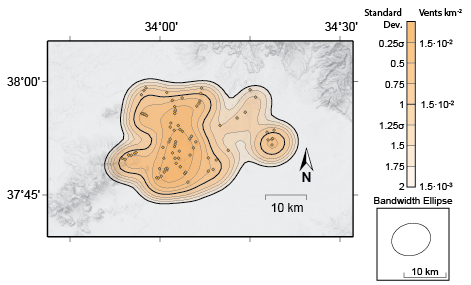
\includegraphics[width=\linewidth]{\FigPath/egrikuyu_kde_72dpi}
    \end{subfigure}
    \begin{subfigure}{0.49\textwidth}
        \centering
        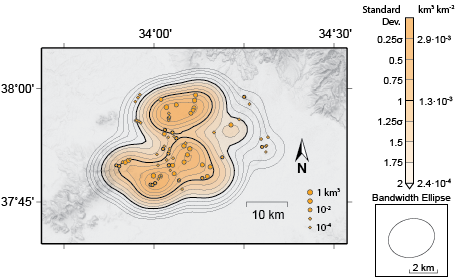
\includegraphics[width=\linewidth]{\FigPath/egrikuyu_vol_72dpi}
    \end{subfigure}
    \caption[Vent density and volume density maps of the E\u{g}rikuyu volcano cluster]{Vent density (left) and volume density (right) maps of the E\u{g}rikuyu volcano cluster. While a large number of vents in the eastern margin of the field make a second mode of vent density, their cumulative erupted volume is much smaller than the volumes erupted from vents in the center of the cluster, so the eastern mode is not seen in the volume density model.}
\label{fig_egrikuyu_kdevol}
\end{figure}

The lava flows that make up the distributed vent field in the Arsia Mons Caldera on Mars also have modeled volumes that correspond to each eruptive event. Figure \ref{fig_arsia_kdevol} shows both the vent density plot of the vent field and the modeled volume distribution. Similar to the E\u{g}rikuyu field, this shows the difference in vent productivity, where the eastern half of the field has vents which produced larger eruptions than the western vents.

\begin{figure}[h!]
    \centering
    \begin{subfigure}{0.49\textwidth}
        \centering
        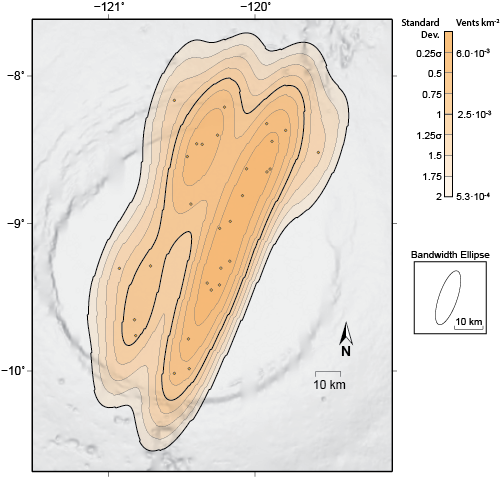
\includegraphics[height=8cm]{\FigPath/arsia_kde_72dpi}
    \end{subfigure} 
    \begin{subfigure}{0.49\textwidth}
        \centering
        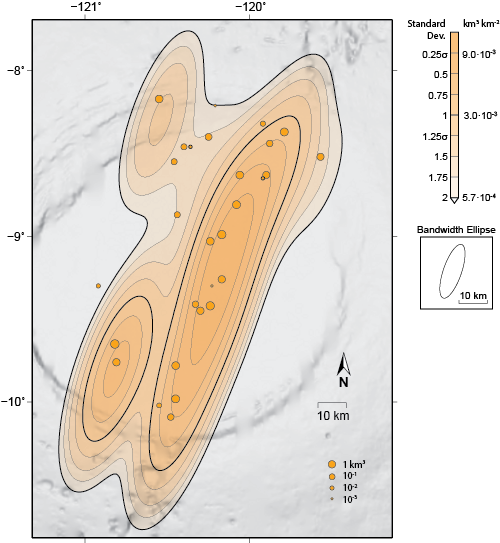
\includegraphics[height=8cm]{\FigPath/arsia_vol_72dpi}
    \end{subfigure}
    \caption[Vent density and volume density maps of the Arsia Mons Caldera volcanic field (Mars)]{Vent density (left) and volume density (right) maps of the Arsia Mons Caldera volcanic field (Mars). Erupted volume density is modeled using minimum volume estimates made using interpolated subsurface models for each volcano. The volume density plot shows that lavas from the east lineament of vents, also visible in the vent density model, are more voluminous than those from the east lineament of vents.}
\label{fig_arsia_kdevol}
\end{figure}

\section{Discussion}
\subsection{Planet-level differences in distributed volcanism}
The major finding of this study is that the spatial intensity of vents between planets is generally different by an order of magnitude. On Earth, six monogenetic volcanic fields cluster on the order of 0.1 vents per km$^2$. On Mars, two clusters have a vent intensity of around 0.001 vents per km$^2$. One cluster, in the basaltic caldera of Arsia Mons, is more focused by a factor of five. In between these vent densities, Venus shield fields have densities of 0.01 vent per km$^2$. Venus shield fields are still more focused than the regional shield plains, which have an average intensity of 0.003 vents per km$^2$, similar to the Arsia Mons cluster. Essentially, volcanic vents in Earth fields have 10s km$^2$ of space between neighboring vents, on Venus, distributed volcanoes have 100s km$^2$ of individual space, and on Mars, two of three fields have 1000s  km$^2$ of space between neighboring vents, while one is clustered on a ``Venusian'' scale (Figure \ref{fig_ventdens}).

There are several reasons to explain this disparity in vent distribution across the inner Solar System. First, it is likely that these different vent intensity scales are influenced by magma focusing or dispersion within the planets' lithospheres. Magma advects upward from a source due to buoyancy and pressure gradients \citep{lister1991fluid}, while it laterally focuses and/or diffuses due to rigidity boundaries and zones of weakness in country rock \citep{hebert2010generation,bonafede1998porous}. If there is a net diffusion effect of magma during ascent through the elastic layer of the lithosphere (the footprint of magma flux at the surface is expected to be larger than the areal extent of the source), then more distributed, areally-larger clusters would be a product of a deeper source, assuming all other factors remain equal. Magma source regions set at the base of the lithosphere's elastic layer of Mars and Earth would be in line with this trend; while the elastic thickness under distributed volcano fields on Earth is generally 20-40~km \citep{kiyosugi2010relationships}, elastic thickness in the Tharsis region on Mars is 60-100~km \citep{neumann2004crustal}. Venus elastic lithospheric thickness is not well constrained \citep{anderson2006global} but might be similar to the thickness on Earth \citep{nimmo1998volcanism}. If there is a net focusing effect of magma during ascent due to regions of more fracturing, Earth's focused fields might be due to its plate tectonic regime, while Venus is less tectonically active and Mars even less so, resulting in less and less focused distributed volcanism.

Second, heat might be able to create batches of magma in smaller regions on Earth than Mars, because the Earth's crust is more chemically heterogeneous again due to tectonics. Because of local regions of more evolved rock in the upper mantle on Earth, the degree of partial melt might be elevated compared to Mars and Venus magma production regions \citep{annen2006genesis}. This would enable a more focused source region to be produced, which would form a more focused volcanic field at the surface. In addition to a more focused magma source region, a denser cluster of dikes in an area of the elastic lithosphere might heat it to an extent that subsequent intrusions are less likely to cool and stall below the surface. If source regions are less productive per square kilometer on Mars and Venus, this thermal feedback might not occur.

The abundance of water within each planet might also affect vent intensity. Water is a primary difference between Earth and Venus: the mantle of Venus is expected to have been dry for at least the last 0.5~Ga, because no mechanism has been identified which returns water to the mantle and because the atmosphere of Venus only contains $<$200~ppm water \citep{donahue1992past,nimmo1998volcanism}. Venus and Earth are similar in other ways: both have comparable masses, the effective elastic thickness within both lithospheres are on the order of 10s~km, and both planets' mantles have potential temperatures of $\sim$1300$^{\circ}$C \citep{nimmo1998volcanism}. The abundance of water is known to play a key role in producing melt and lowering the effective viscosity of the mantle lithosphere on Earth, enabling distributed volcanism in the terrestrial settings presented in this chapter \citep{dixon2004lateral}. On Venus, the dry mantle lithosphere has a higher viscosity than Earth's and melting begins at higher temperatures, which likely decreases the amount of magma able to ascend to the surface. In the elastic lithosphere of Venus, the lack of water effectively strengthens rocks and faults can withstand eight times more stress than faults on Earth \citep{nimmo1998volcanism}. This might inhibit the propagation of dikes. With less magma melting per square kilometer and fewer dikes ascending to the surface, the number of volcanoes being created in a volcanic field will be decreased. The presense of water might therefore be the major factor in producing dense clusters of volcanoes on Earth compared to the more diffuse clusters on Venus.

The distinct differences between the tectonism and magma production of Earth, Mars, and Venus will effect the spatial organization of volcanoes in distributed volcanic fields in overlapping ways. The variation in spatial vent intensity by orders of magnitude between these planets cannot likely be accounted for by one process alone, but the observation of this variation does indicate that distributed volcanism is fundamentally sensitive to tectonic regime and the productivity of magma generation as described above.

%In conclusion, we can't tell, but maybe a combination

%Second half of Chuck comment:
%There is another way to look at this. Distributed volcanic fields on Earth are thought to form because rates of magmatism are too low to sustain a shallow magma chamber, which is frequently replenished by melt form depth. Thus, each ascending dike finds it's own path to the surface. However, dense Earth volcano clusters may be thermally advantageous. That is, a dike is more likely to reach the surface if the lower crust has been pre-heated by previous dikes. 

%Geothermal gradients were likely much higher during periods of active volcanism on Venus (current high search temperatures mean less cooling during ascent) and Mars (demagnetized crust) than  Quaternary earth volcanic fields.  Consequently thermal filtering is a less efficiant mechanism, resulting in a broader distribution of volcano clusters on Mars and Venus. That is, low percentage melting of the mantle on Venus and Mars is more likley to produce melts that reach the surface because the geothermal gradient is higher - they have less chance to cool.

%Although the observation of fundamental diffeences in vent density cannot prove anyone of these processes, the large differences on a planetary scale indicate that processes like the ones discuessed here have caused funadamental differneces in duistributed volcanism on the three planets.



\subsection{Geologic implications of the kernel bandwidth}
Each bandwidth ellipse mimics attributes of its corresponding vent cluster and likely reflects geologic properties which effect the volcano cluster. The bandwidth ellipse area at one standard deviation (1-sigma) reflects both the spatial extent of volcanoes in the cluster and the number of vents in the cluster. Larger volcano clusters correlate with larger bandwidths ellipses, while clusters with more volcanoes in the same amount of space have smaller bandwidths. Because bandwidth area is correlated with these two characteristics, it is better to refer to each characteristic directly. Similarly, bandwidth ellipse elongation, or the difference in the major and minor axis standard deviations, is a function of the anisotropy in vent production through the cluster, either because of a farther extent of volcanoes in one direction or because of more vents per km in one direction. Because of this, the anisotropy of vent production in a cluster can be explored using bandwidth elongation as a proxy.

Elongation of the bandwidth of a volcano cluster can be explained by one or a combination of at least three geologic processes. First, the magma source region underlying the volcano cluster might be elongated, matching the distribution of volcanoes observed at the planet's surface. Second, the magma source region might have migrated with time or multiple magma source regions that are spatially adjacent might be overprinting pre-existing populations. Third, the lateral migration of magma within the elastic lithosphere might itself be anisotropic, preferentially focusing magma in one direction or enabling magma to spread laterally away from a source region. While all three of these might apply to all volcanic fields in varying degrees of magnitude, I will discuss how the anisotropy seen in the bandwidth ellipse might be explained by one of these processes for example clusters. Comparing bandwidth orientation and elongation to different magmatic and tectonic processes might help to explain the relative power of different processes in governing the shape of volcano clusters.

\begin{figure}
\centering
\begin{subfigure}{0.49\textwidth}
\centering
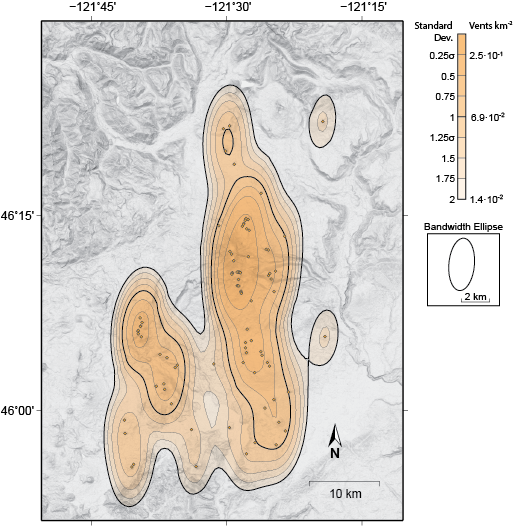
\includegraphics[width=\linewidth]{\FigPath/adams_kde_72dpi}
\end{subfigure}
\begin{subfigure}{0.49\textwidth}
\centering
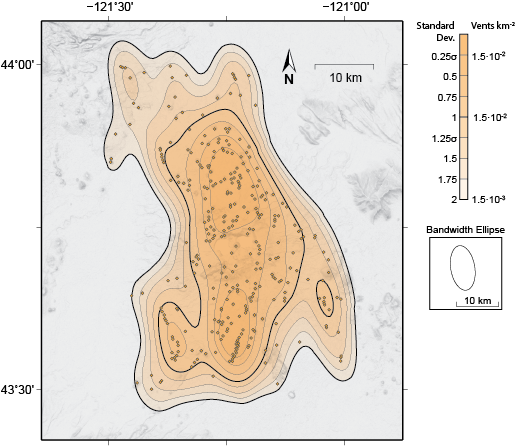
\includegraphics[width=\linewidth]{\FigPath/newberry_kde_72dpi}
\end{subfigure}
\caption[Volcanic vent density of monogenetic volcanoes near Mt. Adams (Washington, USA) and Newberry Volcano (Oregon, USA)]{Volcanic vent density of monogenetic volcanoes near (left) Mt. Adams (Washington, USA) and (right) Newberry Volcano (Oregon, USA). If the magma source region is elongated N-S due to the subduction of the Juan de Fuca Plate to the west, this might result in an elongated volcano distribution and kernel bandwidth ellipse.}
\label{fig_adams-newbkde}
\end{figure}

\subsubsection{Elongated source region}
The bandwidth ellipse of elongated clusters is often elongated in the same direction, such as the ellipse for scoria cones around Mount Adams, Washington (left, Figure \ref{fig_adams-newbkde}). The distributed volcanic field around Mount Adams runs parallel to the Cascades volcanic arc, possibly because the magma source region of the field runs along the axis of the Arc. As can be seen in Figure \ref{fig_earthlocator}}, both Cascades clusters, Adams and Newberry, have kernel bandwidths that are in line with the volcanic arc (Figure \ref{fig_adams-newbkde}). Both Japanese clusters, Abu and Izu-Tobu, also have bandwidths in line with the arc that makes the lower limb of the country's main island, Honshu. For regions where magmatic activity is expected to be elongated, for example rift valleys and subduction zones, it is possible that bandwidth ellipse orientation is primarily due to the elongation of the magma source region \citep{germa2013tectonic}.



\subsubsection{Magma source migration or multiple overprinting sources}
The eastward migration of volcanism in the San Francisco Volcanic Field is observed from magnetic polarity reversals identified in cores taken from volcanoes in the SFVF. The volcano cluster has been active for three magnetic epochs. The most recent volcanoes, including the $\sim$1000 year old Sunset Crater, are located in the eastern portion of the field and were emplaced during a normal-polarity magnetic field \citep{tanaka1986migration}. Volcanic edifices with reverse polarity are located in the center of the field. The oldest volcanoes are to the west and are normally magnetized. \citet{tanaka1986migration} labeled the most recent sub-group the Brunhes group, the reverse-magnetized sub-group the Matuyama group, and the oldest group the pre-Matuyama group. If the geographic centroid of each group is located, an eastward (93$^{\circ}$N) march of the sub-group centroids of 2.9$\pm$0.3 cm/yr can be observed \citep{tanaka1986migration}.

\begin{figure}
\centering
\begin{subfigure}{0.49\textwidth}
\centering
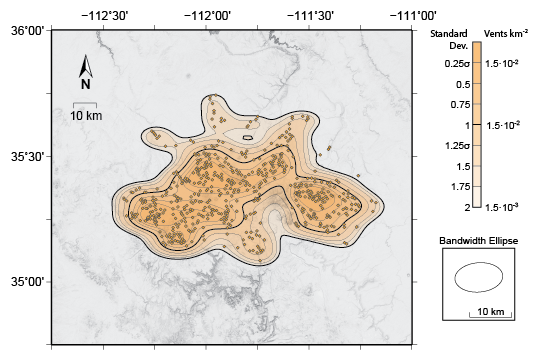
\includegraphics[width=\linewidth]{\FigPath/sanfrancisco_kde_72dpi.png}
\end{subfigure}
\begin{subfigure}{0.49\textwidth}
\centering
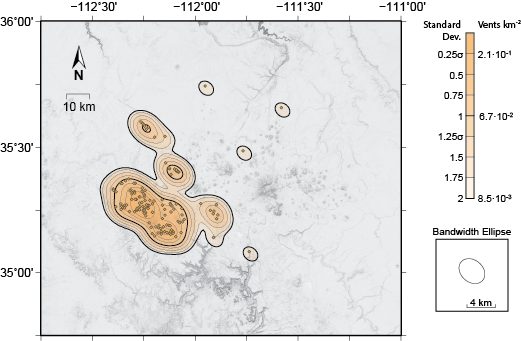
\includegraphics[width=\linewidth]{\FigPath/sanfranciscoP_kde_72dpi.png}
\end{subfigure}
\begin{subfigure}{0.49\textwidth}
\centering
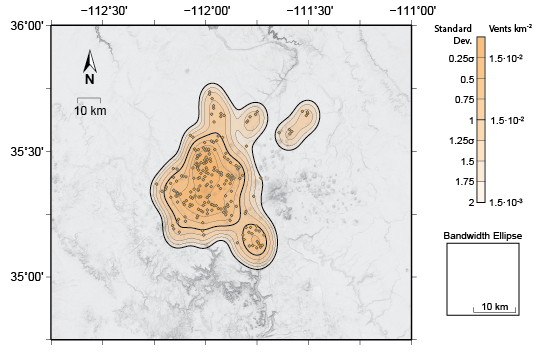
\includegraphics[width=\linewidth]{\FigPath/sanfranciscoM_kde_72dpi.png}
\end{subfigure}
\begin{subfigure}{0.49\textwidth}
\centering
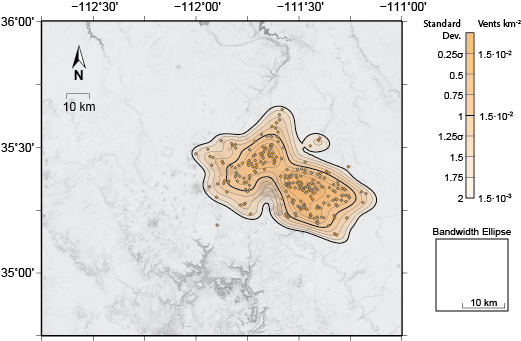
\includegraphics[width=\linewidth]{\FigPath/sanfranciscoB_kde_72dpi.png}
\end{subfigure}
\caption[Vent density through time for the San Francisco Volcanic Field (Arizona, USA)]{Vent density through time for the San Francisco Volcanic Field (Arizona, USA). Top left, the entire volcanic field including 583 vents. Top right, spatial density of vents created during the Pre-Matuyama magnetic chronozone, 5-2.48~Ma \citep{tanaka1986migration}. Bottom left, density of Matuyama-age, 2.48-0.73~Ma vents. Bottom right, Bruhnes-age, 0.73-present, activity. While volcanic activity has migrated eastward, the kernel bandwidth ellipse has also changed. Taking all age vents into account, the bandwidth ellipse is oriented in the direction of migration (top right).}
\label{fig_sfvfkde}
\end{figure}

This eastward march can be compared to the modeled kernel bandwidths of each volcano sub-group (Figure \ref{fig_sfvfkde}). None of the three subgroups' bandwidths are elongated in the direction of the migration identified by \citet{tanaka1986migration}. Bandwidth ellipses of two of the subgroups, the pre-Matuyama and the current Brunhes are elongated in to the northwest, possibly in line with a pre-existing NW-SE fracture set that heavily influences vent geometry  in the field \citep{marshall2015subsurface}. However, the bandwidth ellipse calculated for the entire field is in line with this migration.

Similarly, formation of scoria cones in the Springerville volcanic field is seen to migrate in an ESE direction, 106$^{\circ}$, by 2.5$\pm$0.8 cm/yr. Unlike the San Francisco Volcanic Field, this field is not divided by magnetic epochs, but the group has been divided into two units, older and younger than 1.2~Ma, using K-AR dating and stratigraphy by \citet{condit1989patterns}. Similar to \citet{tanaka1986migration}, the centroids of the two units, together comprised of 230 scoria cones, are used to calculate the velocity of the migration. Like the San Francisco Volcanic Field, the bandwidth ellipse is elongated in the direction of the migration, though not as noticeably as the former.

On Mars, volcanic activity on Syria Planum also migrated over the course of its development. \citet{richardson2013volcanic} identified two major sub-clusters of coalesced shield volcanoes, separated by a large lava flow front of one of the clusters, which embayed volcanoes of the other cluster. The embayment suggests that the southeast group of volcanoes was emplaced first, with crater age-date modeling suggesting an age of 3.4-3.2~Ga. The northwest group was then emplaced between 3.2-2.6~Ga \citep{richardson2013volcanic}. Because of the high uncertainty currently associated with crater age-dating, it is possible that the entire field was emplaced without a migration from the southeast to the northwest. In this case, the bandwidth ellipse (Figure \ref{fig_syriakde}) might be more indicative of the geometry of the magma source region. If, however, there was a migration of magmatic activity or if the two clusters are simply two magmatic events that occured in the same location, the elongation of the bandwidth ellipse would be explained by this migration.

\begin{figure}
\centering
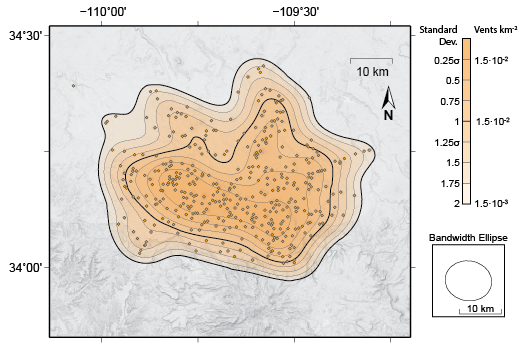
\includegraphics[width=0.6\linewidth]{\FigPath/springerville_kde_72dpi}
\caption[Volcanic vent density of the Springerville Monogenetic Volcanic Field (Arizona, USA)]{Volcanic vent density of the Springerville Monogenetic Volcanic Field (Arizona, USA). The migration of the magma source with respect to the surface over time might be the source of the E-W elongated kernel ellipse.}
\label{fig_springervillekde}
\end{figure}

\begin{figure}
\centering
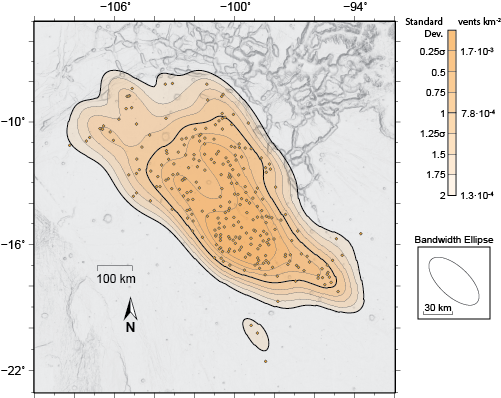
\includegraphics[width=0.6\linewidth]{\FigPath/syria_kde_72dpi}
\caption[Spatial vent density model of Syria Planum (Mars)]{Spatial vent density model of Syria Planum (Mars). A northwest migrating magma source or two overprinting magma sources to the northwest and southeast might explain the elongation of the field.}
\label{fig_syriakde}
\end{figure}


\subsubsection{Anisotropic crustal conductivity}
\citet{bonafede1998porous} modeled the crust under Mount Etna as a porous medium through which pressurized magma can freely flow. In this model, magma migrates based on a hydraulic head pressure and the hydraulic conductivity of the crust. If conductivity is low, magma will flow less, while if conductivity is high, magma will flow more easily through the medium. By modeling an anisotropic conductivity, where conductivity is less or more for magma traveling east or west than for magma traveling north or south, \citet{bonafede1998porous} were able to match the expected surface output of magma to the historical distribution of flank eruptions at Etna. 

Hydraulic conductivity, the ability for fluid to migrate, in the elastic lithosphere can be related to pre-existing fracture sets, as aligned fractures enable magma to propagate more easily in the direction parallel to the fractures \citep{delaney1986field}. Conductivity can also be a product of dynamic stress \citep{germa2013tectonic}, since dikes open in the direction of least compressive stress and propagate in directions normal to the least compressive stress \citep{rubin1995propagation}. 

Magma will be less focused in a direction if magma can laterally propagate in that direction more than other directions. Were the magma source region a point at depth, then the shape of the field might solely be a product of this anisotropic conductivity in the lithosphere's elastic layer. Because the elliptical bandwidth can be used as a proxy for field elongation, directional conductivity differences can potentially be identified by comparing the bandwidth orientation to the direction of geologic features that would increase or decrease crustal conductivity (e.g. direction of crustal strain, pre-existing joints, graben). 

\begin{figure}
\centering
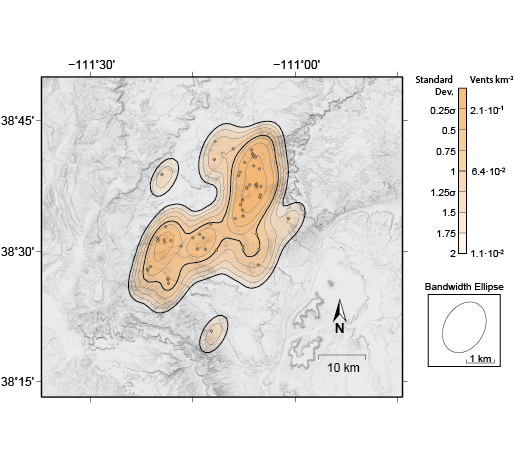
\includegraphics[width=0.6\linewidth]{\FigPath/sanrafael_kde_72dpi}
\caption[Volcanic conduit density of the San Rafael Volcanic Field (Utah, USA)]{Volcanic conduit density of the San Rafael Volcanic Field (Utah, USA). Dikes are oriented north following pre-existing joint sets in the elastic lithosphere, possibly influencing the shape of the kernel ellipse.}
\label{fig_sanrafaelkde}
\end{figure}

The San Rafael volcanic field is one example where existing structural features likely play a significant role in the overall distribution of volcanic vents. The San Rafael Swell has been recently eroded to expose its magma plumbing system \citep{richardson2015sills}. Conduits which formed volcanoes here are mapped in Figure \ref{fig_sanrafaelkde} and are located along dikes as locations where a dike widened to create a conduit diatreme. Dikes in this field are oriented N15W to N, and were likely oriented in this direction by well-developed joints in the Glen Canyon Group: sedimentary rocks underlying the field \citep{delaney1997physical}. The elliptical bandwidth orientation in this field is 30$^{\circ}$N (Figure \ref{fig_sanrafaelkde}), which is not perfectly in line with the dike orientation. However, it is possible that the primary N-S elongation of this bandwidth is due to the joint orientation, while the E-W component can be explained by some other process (e.g. source region geometry).


\begin{figure}
\centering
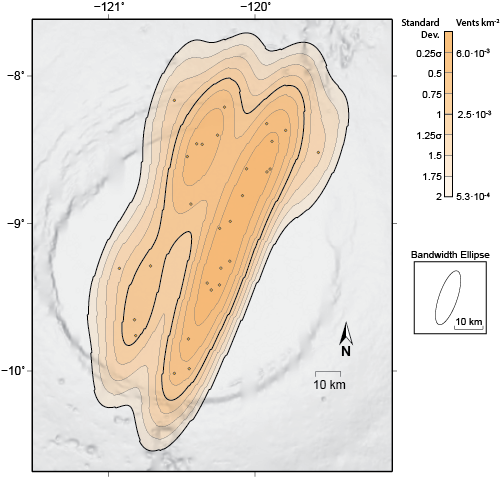
\includegraphics[width=0.6\linewidth]{\FigPath/arsia_kde_72dpi}
\caption[Volcanic vent density of the Arsia Mons Caldera Volcanic Field (Mars)]{Volcanic vent density of the Arsia Mons Caldera Volcanic Field (Mars). Each root of the tooth-shaped density model is parallel with large rift graben that cut the flanks of the volcano.}
\label{fig_arsiakde}
\end{figure}

On Mars, the volcanic field in the Arsia Mons Caldera is also likely shaped by pre-existing fractures in the volcano. Arsia Mons is located at the southern end of the Tharsis Montes and is cut by two large sets of grabens. These grabens are visible on the upper flanks of the mountain but are not visible in the 110~km caldera of Arsia. Instead the caldera is covered by young lava flows that were emplaced from 29 volcanic vents, mapped in Figure \ref{fig_arsiakde}. The density model of the Arsia field is bimodal with two long, parallel lineaments of vents spanning the diameter of the caldera. The orientation of the bandwidth major axis is 19$^{\circ}$N, which is also the orientation of the two graben sets. In addition, the two alignments of vents in Figure \ref{fig_arsiakde} are each in line with one of the rift grabens. This is evidence that dikes creating this vent field would have preferentially ascended parallel to the existing faults.

\section{Conclusions}
The spatial density of volcanic vents in distributed volcano clusters on three different planets has been modeled using Kernel Density Estimation. Vent intensity for clusters appears to be governed on the planetary scale, with vent intensity being highest at Earth clusters (0.1 vents per km$^2$), lowest at Mars clusters (0.001 vents per km$^2$), and intermediate in Venus clusters (0.01 vents per km$^2$). While most clusters have tens to hundreds of vents, Venus shield plains have thousands of vents. Shield plains are also the largest clusters by area, but have similar vent intensity as the shield fields on Venus. The difference between the spatial distribution of volcanoes in clusters on these three planets is likely due to lithospheric characteristics (e.g. elastic thickness, level of fracturing in the upper lithosphere, and water abundance) and tectonic regime, where active tectonism concentrates chemically evolved rocks which melt easier and alters regional stress patterns.

The kernel bandwidths of volcano clusters, or the bivariate normal distributions used to model spatial density, have been calculated using the SAMSE selector \citep{duong2007}, which estimates the bandwidth size assuming the distribution of point features on a map is a random sample of an unknown 2D probability density function. These bandwidths, like the size and vent density of clusters, also are unique to each planet. 

Bandwidth orientation and elongation might also be indicative of underlying characteristics of the elastic layer of the lithosphere or the magma source region itself. Three possible processes might influence bandwidth dimensions: an elongated source region, source region migration, and anisotropic conductivity in the elastic lithosphere that enables or inhibits magma focusing in different directions. While a kernel bandwidth and its corresponding volcano cluster might be influenced by any or all three of these processes, the relative amount that each of these processes influences the cluster formation can be estimated by comparing the bandwidth orientation to hypothesized or known features of the underlying magmatic and tectonic systems.

%%%%%%%%%%%%%%%%%%%%%
%%References Section
%\section{References}

%\nobibliography{dissertation_refs}
%\bibliographystyle{apalike} 

